\documentclass[utf8]{beamer}

\usepackage{beamerthemesplit}
\usepackage{latexsym}
\usepackage{eurosym}
\usepackage[activeacute,spanish]{babel}
\usepackage{ae,aecompl}
\usepackage{graphicx}
\usepackage{amsfonts}


\mode<presentation>{
\usetheme{Warsaw}
\usecolortheme[RGB={20,8,90}]{structure}
\setbeamercovered{transparent}
}

\title{UNA AVENTURA EXTRAÑA Y ESPACIAL}
\subtitle {Proyecto de Python}
\author{ Ricardo Campuzano  Ana Mora Ocaña}
\date{\today}
\institute {ESPOL}

\begin{document}
\begin{frame}[plain]{Lenguajes de programación}
\begin{center}

\includegraphics [width = 0.3 \textwidth]{logo.png} %para colocar el logo de la presentación
\end{center}
\titlepage
\end{frame}

%indice
\begin{frame}
\frametitle{Esquema} %Esquema es el titulo de la diapositiva
\tableofcontents[pausesections]
\end{frame}

\section{Descripción del Proyecto}
\begin{frame}[allowframebreaks]

\begin{block}{Descripción del Proyecto }
El proyecto realizado con la finalidad de ayudar a personas con discapacidad visual, Interactuando con el usuario por medio de sonido y de instrucciones de voz.
 Consiste en narrar una aventura en la cual nosotros mismos le damos el final dependiendo de las opciones que escojamos,todo esto atravez de instruciones de voz
\end {block}
\end{frame}
\section{Descripción de la Aventura}
\begin{frame}[allowframebreaks]

\begin{block}{Descripción de la Aventura }
La aventura se llama "Una aventura Extraña y Espacial" escrita por Enrrique D.Bosch la cual nos narra un sueño muy extraño de un chico que viaja por diferentes mundos.
\end {block}
\end{frame}

\section{¿Comó se realizó?}
\begin{frame}[allowframebreaks]
\begin{block}{¿Comó se realizó? }
El proyecto realizado en Python, con la libreria Pyaudio utilizando como IDE NetBeans 6.9 y para grabar se utilizo Audacity 
\end {block}
\end{frame}

\section{Imagenes}  
\begin{frame}[allowframbreaks]
\frametitle{Imagenes}
\begin{center}

\includegraphics[width=0.5\textwidth]{apli.png}
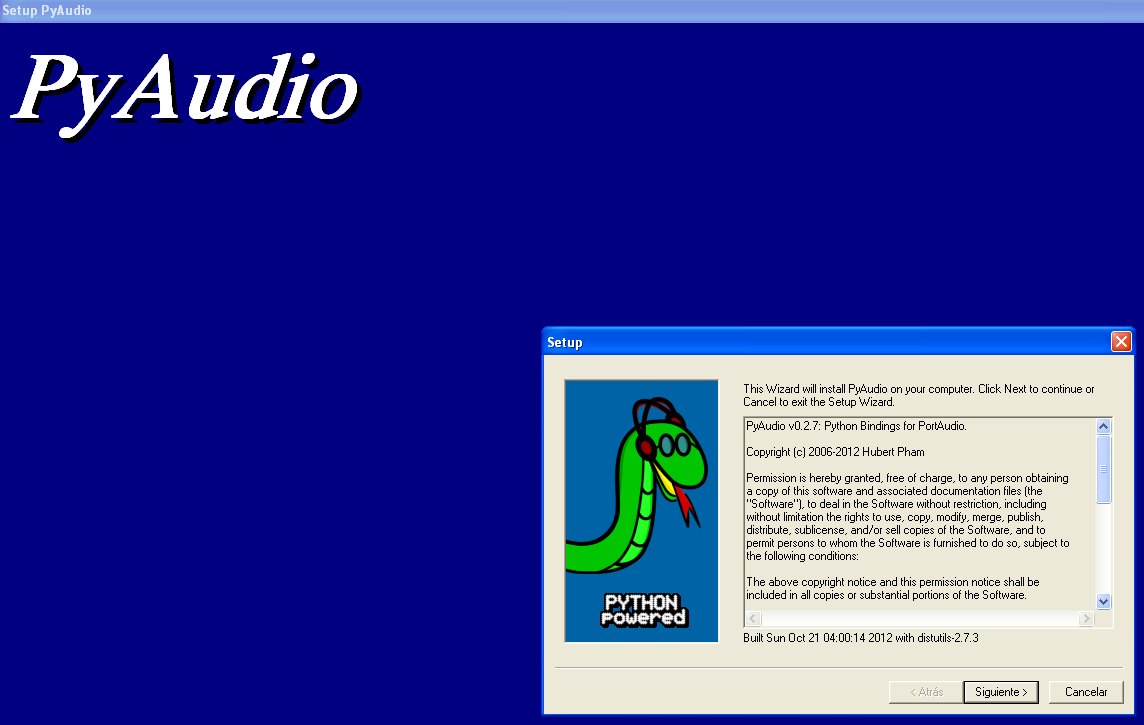
\includegraphics[width=0.5\textwidth]{dibujo.png}
\end{center}
\end{frame}

\begin{frame}[allowframbreaks]
\frametitle{Imagenes}
\begin{center}
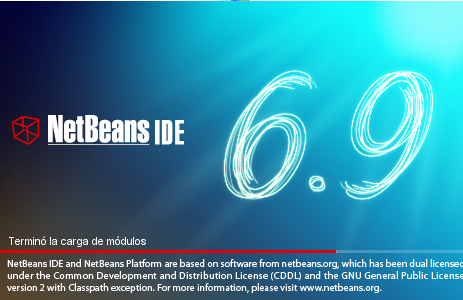
\includegraphics[width=0.5\textwidth]{img1.png}

\includegraphics[width=0.5\textwidth]{img2.jpg}
\end{center}
\end{frame}

\end{document}